\section{Bitlocker}
% https://edk2-docs.gitbook.io/edk-ii-uefi-driver-writer-s-guide/3_foundation/36_protocols_and_handles/365_tag_guid

Our final attack will be targeted against systems using BitLocker \ac{FVE} with a \ac{TPM} 2.0 an no additional PIN or startup key. This leaves the Windows boot partition encrypted, the \ac{ESP} is left unencrypted, thus not affecting the bootkit installation process. Secure Boot can be enabled in combination of BitLocker having the same effects on this attack as described in the second attack \autoref{sec:attack_secure_boot}. Due to the boot- and rootkit still sharing their core functionality we keep the approach abstract and make no further distinctions between the two. We refer to them with the expression \ac{UEFI} payload, not to be confused with our (Windows) payload that is deployed in the Windows installation.

\subsection{Infection}

For the most part of this attack we assume, that the infection is performed after BitLocker has been fully set up, only briefly touching the scenario of a user enabling BitLocker while being infected. When booting with our previous \ac{UEFI} payload, the \ac{NTFS} driver is unable to recognize any file system structure  on the Windows boot partition, due to the \ac{FVE}. Resulting in an inability to further deploy the Windows payload on the target system. Additionally, during execution of the Windows Boot Manager, the BitLocker recovery prompt, shown in \autoref{fig:bitlocker-recovery-prompt}, interrupts the regular boot process requiring the drive's recovery key for decryption before being able to continue booting.
% tpm values differ
% measured pcrs
% not unsealing vmk with tpm
This happens due to \ac{TPM} \ac{PCR} values differing from what was initially used to seal the \ac{VMK}, leaving the Windows bootloader unable to retrieve an unencrypted \ac{VMK} from the \ac{TPM} and as a result unable to decrypt the Windows installation \cite[12.]{windows-internals-7-part2}.

\begin{figure}[htb]
    \centering
    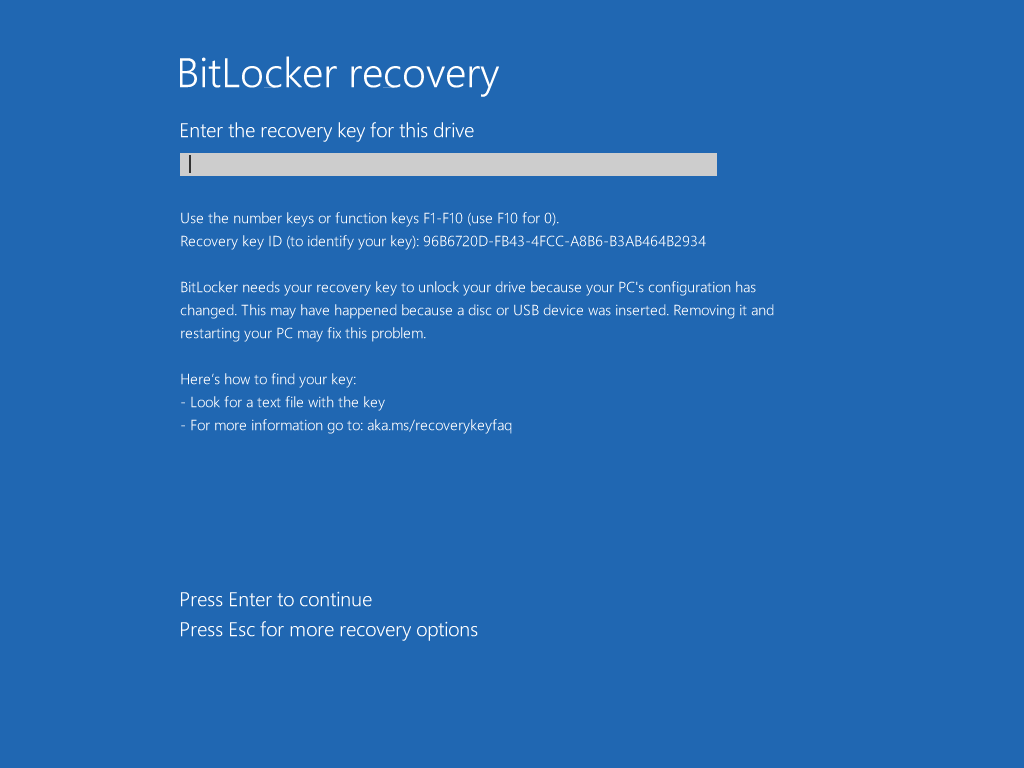
\includegraphics[width=1.0\textwidth]{attacks/bitlocker/bitlocker_recovery_prompt.png}
    \caption{BitLocker Recovery Prompt}
    \label{fig:bitlocker-recovery-prompt}
\end{figure}

In theory this is as far as we get, BitLocker in combination of \ac{TPM} measurements successfully mitigates \ac{UEFI} attacks by discovering a deviation in the boot flow.
% what is the reaction of the average user
In practice we have to ask ourselves the question how a user reacts to seeing the BitLocker recovery prompt and the consequences to the action the user takes. As an immediate reaction the user has two options: entering the recovery key into the prompt or not entering the recovery key.
% motivation behind user decision
What decision the user makes is dependent on their tech savviness and influenced by a variety of factors such as urgency of booting into Windows, knowing alternatives to what the prompt tells them.
It is reasonable to assume that the average user is willingly entering their recovery key in response to the prompt as the prompt does not suggest any malicious causes or any negative repercussions in following the instructions. The link mentioned in the prompt also only aids in locating the recovery key \cite{microsoft-recovery-key-faq}.
\TODO{mention microsofts reasons for the prompt to be triggered}
\TODO{what is the actual alternative}
% does the user trust the system
% why would they not trust the system
% (ask admin for recovery password)
% type in recovery password
% alternative would be to remove drive and insert into safe device



\subsection{Approach}

When the user enters their recovery key the Windows Boot Manager uses the recovery key to decrypt the \ac{VMK} meta data entry, that was encrypted using the recovery key when BitLocker was set up. It then proceeds to access the bitlocked NTFS drive containing the \lstinline{Windload.efi} \ac{OS} loader. This all still happens in the UEFI boottime environment, before \lstinline{ExitBootServices} was called. Unfortunately we are still unable to access the Windows installation, as BitLocker only ever decrypts read operations in memory, leaving the drive fully encrypted at all times.

\subsubsection{BitLogger}

If we were to acquire the recovery key, we could use it to decrypt the \ac{VMK}, the \ac{FVEK} and in turn the drive ourselves. We can simply log the keystrokes performed by the user when entering the key during the recovery prompt. Since we still are in the \ac{UEFI} boottime environment, the Windows Boot Manager uses \ac{UEFI} protocols for user input. \ac{UEFI} offers two protocols for this purpose the \emph{Simple Text Input Protocol} and the \emph{Simple Text Input Ex Protocol}, we can quickly determine which of these is used by the Windows Boot manager by adding a simple \lstinline{print} statement to the implementation in the \ac{OVMF} source code, this change alone triggers the recovery prompt bcause of \ac{PCR} value changes. A keystroke now shows us that the \emph{Simple Text Input Ex Protocol} is being used, the protocol structure is depicted in \autoref{lst:simple-text-input-ex-protocol}. The Windows Boot Manager uses the \lstinline{ReadKeyStrokeEx} function to retrieve the latest pending keypress. The protocol offers the \lstinline{WaitForKeyEx} event, signaling when keystrokes are available, execution can be blocked until this event is emitted with the \lstinline{WaitForEvent} Boot service.


\lstinputlisting[language=C,caption={Simple Text Input Ex Protocol Structure},captionpos=b,label=lst:simple-text-input-ex-protocol]{code/simple_text_input_ex_protocol.h}

We can intercept the \lstinline{ReadKeyStrokeEx} function call by using a technique called function hooking, there are various ways of doing this, for example patching a jump instruction at the beginning of the target function to detour the execution flow. \TODO{if we have time talk about downsides of function patching} \ac{UEFI} protocol hooking does not require such an invasive technique. When we take a closer look at how protocols are returned to their user we can see why. The \ac{UEFI} Boot Services offer two functions, \lstinline{HandleProtocol} and \lstinline{OpenProtocol}, that can be used to retrieve a protocol instance, the latter additionally keeps track of the protocol users \cite[7.3. EFI_BOOT_SERVICES.OpenProtocol()]{uefi-spec}, \autoref{lst:handle-protocol} shows how \lstinline{HandleProtocol} can be used to receive the \emph{Simple Text Input Ex Protocol} instance installed on the active console input device \cite[4.3 EFI System Table]{uefi-spec}. The input paremeters are a device handle, the \ac{GUID} identifying the protocol and the address of a pointer to the protocol structure. When calling \lstinline{HandleProtocol} the value of the pointer is modified to point to the corresponding protocol instance. The protocol instance itself is previously allocated by a driver and installed onto the device handle in their Driver Binding Start function \TODO{Driver binding}. The driver assigns the function fields with functions residing in the driver's image. This is why it is important for a driver's image to remain loaded even after initial execution. The important fact about this process is, that a driver installs only one protocol instance per device handle and every protocol user receives the same address for this protocol instance, given they use the same device handle. Since our \ac{UEFI} payload is executed before the Windows Boot Manager we can query all instances of the \emph{Simple Text Input Ex Protocol} and change the function pointer of \lstinline{ReadKeyStrokeEx} to point to our function hook. When a user later receives a pointer to the protocol instance, accessing the \lstinline{ReadKeyStrokeEx} field will cause our hook to be called instead of the original function. The hook has to be implemented in a driver, so that it remains loaded until the Windows Boot Manager uses \lstinline{ReadKeyStrokeEx}. We also have to save the original function address, together with a pointer to the protocol instance, so that we can call it later. Multiple different drivers could offer the same protocol, resulting in different functions being called depending on the device, the protocol instance is retrieved from. When our hook is called we start by identifying which original function needs to be called using the protocol instance that is used as the first argument of the \lstinline{ReadKeyStrokeEx} function signature. We then call the original to read the pending keystroke, keeping track of the keystrokes (separately for each protocol instance), before returning the key data back to the caller. We coin this BitLocker specific keylogger \emph{BitLogger}.

\lstinputlisting[language=C,caption={Example usage of the \lstinline{HandleProtocol} Boot service},captionpos=b,label=lst:handle-protocol]{code/handle_protocol.c}

The BitLocker recovery prompt does not allow the user to input any
\TODO{key input advancement is weird and makes tracking tricky}
F keys
block validity
only divisable by 11
\cite[9. BitLocker Key Recovery]{windows-internals-6-part2}
cursor can move out of incomplete or valid blocks
up and down increments or decrements the cursor position

\subsubsection{Dislocker}

To make use of the recovery key we can use an open source software called \emph{Dislocker}, which implements the \ac{FUSE} interface to offer mounting BitLocker encrypted paritions under Linux for read and write access \cite{dislocker}.

\begin{figure}[htb]%
    \centering
    \includesvg{dislocker_volume_access_stack.drawio.svg}
    \caption{Dislocker Volume Access Protocol Stack}%
    \label{fig:dislocker_volume_access_stack}%
\end{figure}

\begin{figure}[htb]%
    \centering
    \includesvg{dislocker_volume_access_stack_real.drawio.svg}
    \caption{Dislocker Volume Access Protocol Stack}%
\end{figure}


dislocker linux utility
\cite{dislocker}
mount encrypted drive with decryption mean
read and write access
dual boot in vm
enter recovery key and it works
port to\ac{UEFI}

bitlocker encrypts block-wise

% blk and fs
\TODO{explain block devices}
\TODO{explain file system independent abstraction better}
\ac{UEFI} protocol stack
\TODO{diagram of block io, disk io, simple file system and file protocol interaction (with hindsight of adding dislocker beneath block io)}
\cite[13.3.2 Partition Disocvery]{uefi-spec}
Drivers providing \emph{Simple File System Protocol} use the \emph{Block I/O Protocol} to access the underlying media.


hook block io
again hook data mapping

% execute after NTFS driver by doing it in an ExitBootServices hook
It is beneficial for us to write our payload to the Windows installation as close to the end of the \ac{UEFI} environment as possible, this will maximize the presence of drivers and their offered access to hardware devices. It is also a wise design decision for the attacks following to this one. The call of the function \lstinline{ExitBootServices} marks the point of transitioning from boot time to runtime where the operating system takes over the control of the system, it presents a good opportunity for us to perform the write action of our rootkit.
% was muss man beachten bei exitbootservices hooking
\cite{exitbootservices-hooking}
hook ExitBootServices
enable hook
write payload
import registry key
disable hook

next boot would require to recovery key again
% https://learn.microsoft.com/en-us/windows/security/information-protection/bitlocker/bitlocker-use-bitlocker-drive-encryption-tools-to-manage-bitlocker
update tpm values in payload
\cite{microsoft-bitlocker-manage-bde}
caveat pin? look into this


\subsubsection{BitLocker post Infection}
% reference to rootkit definition
persistence when part of root of trust
fresh install / tpm update values
% paper von betreuern
hook \ac{TCG2} Protocol \cite[6.7.3]{tcg-efi-protocol-spec}
\ac{TPM} communication
% \cite[12.7 TPM_Unseal]{tcg-tpm-library-part3-commands}
receive bitlocker \ac{VMK} key and send to dislocker
\cite{bde-format-spec}
\cite{tpm-sniffing}

% https://labs.withsecure.com/publications/sniff-there-leaks-my-bitlocker-key